\section{\eps: Definition, Construction, and Localization}
\label{sec:epsilon}

\subsection{Per-token entropy}
\label{subsec:per-token}

For each generated token $t$, the API returns top-$k$ candidates with
log-probabilities $\ell_1, \dots, \ell_k$. Let
$p_j = \exp(\ell_j) / \sum_j \exp(\ell_j)$ be the renormalized
distribution. Define
\begin{equation}
    \eps_t \;=\; -\frac{1}{\log k} \sum_{j=1}^{k} p_j \log p_j
    \;\in\; [0,1].
    \label{eq:eps}
\end{equation}
Normalization by $\log k$ maps a one-hot distribution to $0$ and a
uniform distribution to $1$. We use $k=5$ (the OpenAI cap), which
covers the dominant mass for code tokens; tails beyond top-$5$ are
negligible for the binary flag decision. The name is deliberate: in
numerical analysis, $\eps$ denotes a small perturbation that
propagates through a computation --- a high-\eps token is such a
perturbation at a specific decision point.

\subsection{Three types of code-generation uncertainty}
\label{subsec:types}

Raw per-token entropy, applied naively, produces too many false
positives to be useful: the bulk of high-entropy tokens in generated
code are not risk indicators. Understanding which ones are, and why,
is what drives the filtering design in the rest of this section.
Empirical analysis of our calibration benchmark reveals three
categorically distinct types of token-level uncertainty in generated
code.

\paragraph{Type 1 --- Cosmetic (naming).} Uncertainty about what to
\emph{call} something (\texttt{sort\_list} vs.\ \texttt{sort\_numbers}).
\eps reaches $0.7$--$0.9$, but any choice is correct. Dominates
\textsc{low} prompts: the top flag on $9$ of $10$ \textsc{low} prompts
was a function or parameter name on the first line.

\paragraph{Type 2 --- Consequential (API/library decisions).}
Uncertainty about which \emph{API or library} to use, e.g.\
\texttt{stripe.Charge.create()} vs.\
\texttt{stripe.PaymentIntent.create()} at the attribute token.
This is the target signal.

\paragraph{Type 3 --- Implementation-approach.}
Uncertainty among multiple correct algorithms (recursive vs.\
iterative Fibonacci, for-loop vs.\ comprehension, brute vs.\ hash-%
based two-sum). \emph{The Type 2 / Type 3 distinction is
definitional, not structural.} A given high-\eps token is classified
as Type 3 precisely when all of the competing continuations produce
functionally correct code; it is classified as Type 2 when at least
one continuation is wrong. The underlying decoder state can look
identical in both cases --- a $0.5$-peaked top-$2$ distribution at a
decision point --- and \eps has no way, from the token distribution
alone, to know which label applies. The label is a property of the
external world (are all branches correct?) and is only visible via
ground truth. Consequently the residual Type 3 false-positive rate
is irreducible at the signal level: a perfect classifier in a world
where both \texttt{list.sort()} and \texttt{sorted(list)} are correct
cannot help firing on the choice. What the system can do is not
\emph{suppress} the fire but \emph{resolve} it: Type 3 false
positives are fast for the stage-2 reviewer to clear because both
alternatives pass inspection.

\begin{table}[h]
\centering
\small
\begin{tabular}{c p{2.4cm} p{6.4cm} p{2.2cm} p{1.2cm}}
\toprule
\textbf{Type} & \textbf{Label} & \textbf{Source} & \textbf{\eps fires?} & \textbf{Risk} \\
\midrule
1 & Cosmetic & Naming choices (\texttt{sort\_list} vs.\ \texttt{sort\_numbers}) & Yes (0.7--0.9) & None \\
\multicolumn{5}{l}{\quad\small\textit{Filter: AST declaration filter removes this uncertainty before scoring.}} \\[4pt]
2 & Consequential & API / library decisions (\texttt{Charge} vs.\ \texttt{PaymentIntent}) & Yes (0.5--0.9) & \textbf{High} \\
\multicolumn{5}{l}{\quad\small\textit{Target signal: this is what the system is designed to catch.}} \\[4pt]
3 & Implementation & Algorithm structure where all branches are correct (recursive vs.\ iterative) & Yes (0.3--0.7) & None \\
\multicolumn{5}{l}{\quad\small\textit{Definitional Type 3: classified Type 3 because all continuations work.}} \\
\bottomrule
\end{tabular}
\caption{The three-type uncertainty taxonomy. Type 2 vs.\ Type 3 is
a property of the target world (are the alternatives all correct?),
not of the decoder state. \eps cannot distinguish them from the token
distribution alone; the stage-2 reviewer resolves them by inspecting
the alternatives.}
\label{tab:taxonomy}
\end{table}

With this taxonomy in hand, the filter design follows directly:
remove Type 1 syntactically, leave Type 3 as a known floor that the
reviewer is cheap to clear, and isolate Type 2.

\subsection{AST filtering}
\label{subsec:ast}

We eliminate Type 1 via the generated code's AST. After stripping
markdown fences and parsing with Python's \texttt{ast}, we identify
\emph{declaration positions} --- source ranges where the model is
choosing a name rather than an API.
\textbf{Filtered:} function/method names, parameter names
(\texttt{ast.arg}), local variable names (\texttt{ast.Name} in
\texttt{Store}).
\textbf{Retained:} import targets, attribute accesses, keywords,
type annotations. Token-to-declaration matching uses range overlap
(BPE introduces a leading space); a pure-identifier guard prevents
over-filtering of delimiter-prefixed tokens such as \texttt{(db}.

\begin{table}[h]
\centering
\small
\begin{tabular}{lcc}
\toprule
\textbf{Configuration} & \textbf{\textsc{low} FP} & \textbf{\textsc{high} det.} \\
\midrule
Naive token entropy (no filtering)                & $100\%$ & $100\%$ \\
+ Whitespace / comment filtering                  & $100\%$ & $100\%$ \\
+ System prompt naming conventions                &  $70\%$ &  $95\%$ \\
+ AST declaration filtering                       &  $60\%$ &  $80\%$ \\
+ Fence-format stripping                          &  $50\%$ &  $80\%$ \\
\midrule
Residual (Type 3 only)                            &  $50\%$ & --- \\
\bottomrule
\end{tabular}
\caption{Successive filtering stages on $10$ \textsc{low} and $20$
\textsc{high} prompts (GPT-4o, fresh staging run). \textsc{low} FP
is the fraction of pure-logic prompts that fired; \textsc{high} det.\
is the fraction of API-version-split prompts that fired. The AST
declaration filter trades a $15$pp drop in \textsc{high} detection
($95\%\to80\%$) for a $10$pp reduction in \textsc{low} FP
($70\%\to60\%$): three \textsc{high} prompts whose peak-$\eps$ token
was a function name (not an API selector) fall below the flag threshold
once declarations are removed. This is correct behaviour --- those
functions were uncertain about \emph{naming}, not about \emph{which
API to call} --- but it is an honest trade-off rather than a free win.
Residual $50\%$ \textsc{low} FP is Type 3 (irreducible); stages
$1$--$2$ use a bare system prompt without naming-convention
instructions.}
\label{tab:filtering}
\end{table}

\subsection{Aggregation: function-level max}
\label{subsec:aggregation}

We aggregate with
$\eps_\text{file} = \max\{\eps_t : t \text{ retained}, \eps_t >
\delta\}$, $\delta = 0.30$. The compound alternative $1 - \prod(1 -
\eps_t)$ converges to $1.0$ for any non-trivial function. Across all
$90$ runs of the benchmark ($3 \times 30$), max and mean produced
identical fire/no-fire decisions at every threshold; we prefer max
because \emph{it preserves the token identity}, not just the
function-level score. A mean would give a reviewer one number; a
max plus the argmax gives a reviewer a specific token to look at.
The contrast with the sequence-level mean token probability baseline
(\papg) is deliberate: averaging over every token dilutes a single
uncertain decision and, more importantly, discards the information
that would tell a reviewer where to look. We revisit this choice
empirically in \S\ref{sec:comparison}.

\subsection{Thresholds and tiers}
\label{subsec:tiers}

Three tiers: \textsc{complete} ($\eps < 0.30$), \textsc{flagged}
($0.30 \le \eps < 0.95$), \textsc{paused} ($\eps \ge 0.95$). The
load-bearing boundary is the binary \textsc{complete} vs.\
\textsc{flagged+}: everything \textsc{flagged+} is forwarded to the
stage-$2$ reviewer. \textsc{paused} is a higher-urgency signal
within the flagged region. These are UX signals, not
calibrated probabilities --- the \textsc{flagged} empirical failure
rate is $\sim 27\%$ (\S\ref{sec:evaluation}).

\subsection{Token-level focus: the distinguishing claim}
\label{subsec:token-focus}

The function-level flag rate answers the question ``which functions
need scrutiny.'' For \textsc{high} prompts it says ``essentially all
of them''; a reviewer given only the function-level signal is told
little more than ``re-read the function.'' The token-level view is
where \eps becomes actionable.

Let $N_f$ be the number of retained (AST-filtered, non-cosmetic)
tokens in a function, and let $N_f^{\ge\tau}$ be the count of those
tokens with $\eps_t \ge \tau$. The \emph{focus ratio} at threshold
$\tau$ is
\begin{equation}
  \rho_\tau(f) \;=\; N_f^{\ge\tau} \,/\, N_f.
  \label{eq:focus}
\end{equation}
$\rho_{0.30}$ is the fraction of semantic tokens that exceed the
flag threshold. We report $\rho$ at the flag threshold because that
is the boundary at which the stage-$2$ reviewer is directed to
inspect a token; the \textsc{paused} function-level threshold
($\eps \ge 0.95$) is near-empty at the token level on this corpus
(only $2$ tokens across $144$ entries cross it, so the rate is not
a useful data point).

\begin{table}[h]
\centering
\small
\begin{tabular}{lrrr}
\toprule
 & \textbf{Fn-level} & \textbf{\eps $>0.30$}
   & \textbf{Tokens@flag} \\
\textbf{Set}
 & \textbf{flagged} & \textbf{(tokens)}
 & \textbf{per fn} \\
\midrule
\textsc{high} ($n=104$) & $97.1\%$ & $10.5\%$ & $10.4$ \\
\textsc{low} ($n=40$)   & $90.0\%$ & $13.1\%$ & $10.4$ \\
\bottomrule
\end{tabular}
\caption{Function-level flagging vs.\ token-level focus across four
models (GPT-4o, GPT-4o-mini, GPT-4-turbo, DeepSeek V3), 30 prompts,
$144$ entries total. The function-level flag rate is near-saturating
on \textsc{high} prompts; the token-level focus narrows the
within-function review surface to $10.5\%$ of the function at the
flag threshold. Average function size is $\sim 98$ retained semantic
tokens. Token review burden reduction at the flag threshold: $89\%$.}
\label{tab:token-focus}
\end{table}

The numbers in Table~\ref{tab:token-focus} are the central
quantitative claim of this paper. A developer reviewing an AI-%
generated function does not face a $98$-token problem. They face an
$\sim 10$-token problem at the flag threshold --- the tokens \eps
identified as high-entropy. The function-level flag rate of $97\%$
is not a problem to be defended against; it is the entry point to a
localization step that no sequence-level aggregate produces and that
prior token-level visualizations~\cite{palacio2024astrust,vasconcelos2024genprob}
provide only as standalone artifacts rather than as routing into a
review loop.

Figure~\ref{fig:token-focus-detail} shows the token-level \eps
trajectory on Stripe Scenario A (GPT-4o). Of $98$ retained tokens,
$10$ exceed the flag threshold. The highest-\eps tokens cluster on
the \texttt{.Ch} method selector on \texttt{stripe} (the
Charge-vs-PaymentIntent decision) and one immediately adjacent
token. The remaining tokens are confident parameter construction,
imports, and return-value handling. A reviewer given this figure
does not re-read the function; they look at the highlighted tokens.

\begin{figure}[H]
\centering
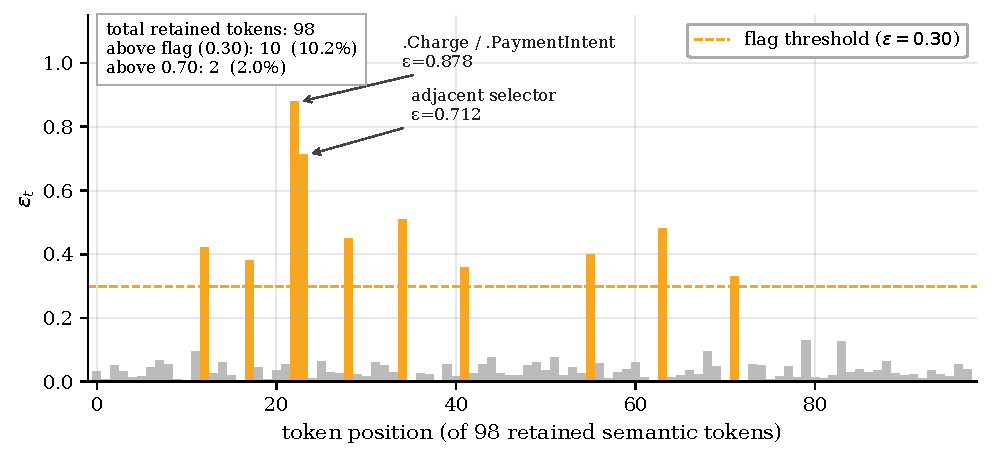
\includegraphics[width=0.85\textwidth]{figures/fig_token_focus_detail.pdf}
\caption{Per-token \eps trajectory, Stripe Scenario A (GPT-4o, $98$
retained tokens). The flag threshold ($0.30$) is dashed. Ten tokens
exceed the flag threshold; the peak localizes to the method-selector
decision between \texttt{Charge} and \texttt{PaymentIntent}. The
rest of the function is confident boilerplate. \eps does not just
flag the function --- it names the tokens that drove the flag.}
\label{fig:token-focus-detail}
\end{figure}

\subsection{Multi-model calibration at a glance}
\label{subsec:calibration-preview}

\eps at the \textsc{flagged} threshold fires on \textsc{high} prompts
much more often than on \textsc{low} prompts. Across four models
(GPT-4o, GPT-4o-mini, GPT-4-turbo, DeepSeek V3), \eps achieves
$70$--$85\%$ \textsc{high} detection at $50$--$70\%$ \textsc{low}
false-positive rate. A detailed calibration table appears in
\S\ref{subsec:calibration}.

\subsection{Adaptive ensemble}
\label{subsec:ensemble}

The production implementation refines tier placement within
\textsc{flagged+} using a rolling mean-\eps baseline and a top-$1$
logprob check; neither affects the binary \textsc{flagged+} gate.
Conformal calibration is left to future work. The current thresholds
($\eps \ge 0.30$ for \textsc{flagged}, $\eps \ge 0.95$ for
\textsc{paused}) are calibrated empirically on GPT-4o and inherited
by other models without formal coverage guarantees. A natural
defense path is split conformal prediction over per-token entropy
scores in the style of TECP~\cite{xu2025tecp}, which would convert
the flag threshold into a coverage-controlled decision (e.g., $90\%$
coverage of the tail of token-entropy values on a held-out
calibration set). The current evaluation supports the thresholds as
UX signals with measured failure rates; statistical guarantees are a
complementary calibration step, not a replacement for the empirical
evidence.
